\documentclass[11pt]{article}
\usepackage[margin=1in]{geometry}
\usepackage{amsmath,amssymb}
\usepackage{booktabs,longtable,tabularx,array}
\usepackage{enumitem}
\usepackage{xcolor}
\usepackage{hyperref}
\usepackage{tikz}
\usetikzlibrary{arrows.meta,positioning,fit,shapes.geometric,backgrounds,calc}
\usepackage{graphicx}

\hypersetup{
  colorlinks=true,
  linkcolor=blue!60!black,
  urlcolor=blue!60!black,
  citecolor=blue!60!black
}

\setlist[itemize]{leftmargin=1.6em}
\setlist[enumerate]{leftmargin=1.8em}
\renewcommand{\arraystretch}{1.15}

\newcommand{\vdt}{\textsc{VDT}}
\newcommand{\barname}{\textsc{VDT-BAR}}
\newcommand{\vcdr}{\textsc{VDT-VCDR}}
\newcommand{\vanilla}{\texttt{vanilla\_dev}}

\title{\textbf{VDT Research Roadmap}\\From Same-Stack Attribution to a Paper-Ready Depth-Routing Story}
\author{Repository-grounded roadmap for the current \texttt{vdt\_dev/} research stack}
\date{\today}

\begin{document}
\maketitle

\section{Project Status and Real Code Boundaries}

The repository currently supports two distinct roles.

\begin{itemize}
  \item The root baseline remains the preserved original \vdt{} reference line. The baseline training and evaluation logic still live in \texttt{main.py}, \texttt{decision\_transformer.py}, \texttt{trajectory\_gpt2.py}, \texttt{src/iql.py}, \texttt{src/util.py}, and \texttt{src/value\_functions.py}. This path should continue to serve reproduction, not rapid research iteration.
  \item The research line now lives inside \texttt{vdt\_dev/} and is already a real experiment platform rather than a loose prototype.
\end{itemize}

The \texttt{vdt\_dev/} stack has progressed through four concrete stages:

\begin{enumerate}
  \item \textbf{Step 1: \barname{}.} The actor backbone adds static-query Block Attention Residual routing over transformer depth. The change is intentionally narrow: actor residual aggregation changes, but the Q/V objectives, actor loss, and original value-guided sampling semantics do not.
  \item \textbf{Step 2: \vcdr{}.} The BAR path now supports four query modes: \texttt{static}, \texttt{state}, \texttt{state\_rtg}, and \texttt{state\_rtg\_value}. Query fusion is additive, \(q = w + \Delta q\), and the value-conditioned mode only uses detached scalar \(V(s_t)\). The repository still does \emph{not} implement advantage-, uncertainty-, or Q-conditioned routing.
  \item \textbf{Step 3: experiment and analysis infrastructure.} \texttt{vdt\_dev/runner.py} now supports manifests, structured logs, best/latest checkpoints, resume behavior, RTG-grid reevaluation, aggregation, plotting, table export, and routing-debug collection. The experiment registry and preset layer already cover query-mode sweeps, depth sweeps, seed sweeps, Gym environment sweeps, and RTG-grid analysis.
  \item \textbf{Step 4: attribution, rigor, and stronger setting.} The repo now includes a same-stack \vanilla{} baseline, compute-reporting plus approximate matched-budget depth presets, and a dev-stack offline-to-online tuning path for Hopper. This gives the project a much stronger paper framing than a pure architecture tweak inside offline Gym-only experiments.
\end{enumerate}

Important real boundaries remain:

\begin{itemize}
  \item \texttt{runner.get\_env\_metadata()} currently supports the Gym medium trio: Hopper, Walker2d, and HalfCheetah.
  \item Maze2D and AntMaze exist only as preset/config templates, not as runnable mainline experiments in the current runtime path.
  \item The matched-budget infrastructure is parameter-matched and compute-aware, but not exact FLOP-matched.
  \item The online path is real and integrated, but the explicit configs and launchers are currently Hopper-first rather than broad-environment online sweeps.
\end{itemize}

The dev test suite is also nontrivial. The current repository contains tests for BAR/VCDR forward and backward behavior, query-conditioning modes, same-stack \vanilla{} support, compute reporting, preset expansion, schema stability, plot smoke tests, and online rollout shape handling. That is important for paper execution because it means the stack is stable enough to support systematic experimentation.

\section{Main Conference Narrative}

\subsection{One-sentence thesis}

Value guidance in \vdt{} should not stop at objectives and target returns; it should also determine which \emph{depth-level representations} the decision model relies on when choosing actions.

\subsection{Three-sentence abstract-level story}
\begin{figure}[htbp]
    \centering
    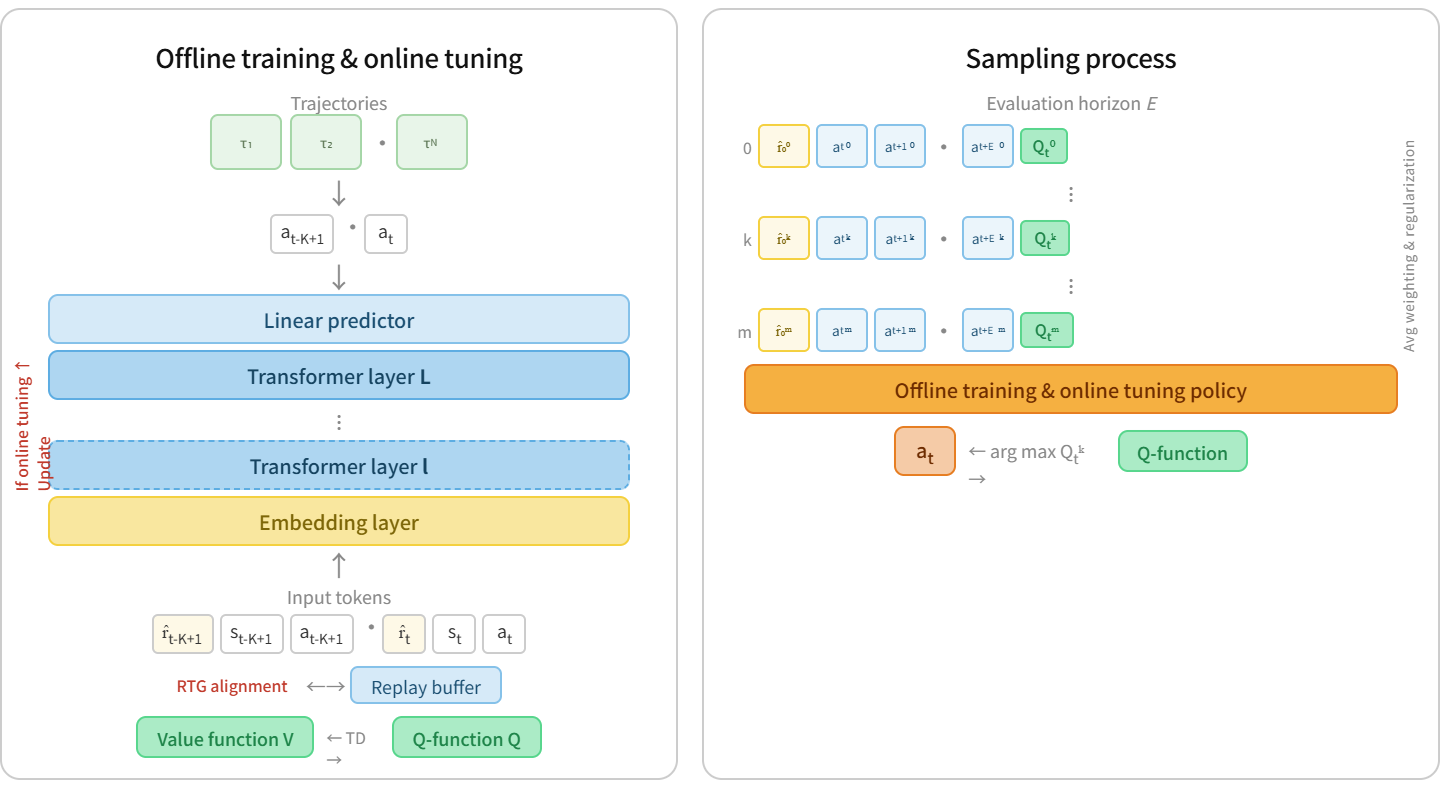
\includegraphics[width=0.8\textwidth]{vdt.png}
    \caption{vdt.png}
\end{figure}

The original \vdt{} already uses value information in the critic/value objectives and in target-return-guided decision making, but it still aggregates transformer depth in a standard residual manner. This project asks whether the actor should also perform \emph{depth-wise residual routing}, first with static routing over grouped residual sites (\barname{}) and then with state/RTG/value-conditioned routing (\vcdr{}), while keeping the original Q/V objectives and sampling semantics fixed. The resulting same-stack comparison---\vanilla{} vs.\ BAR vs.\ VCDR---is the cleanest path to attributing gains to depth routing itself rather than to unrelated training changes.

\begin{figure}[htbp]
    \centering
    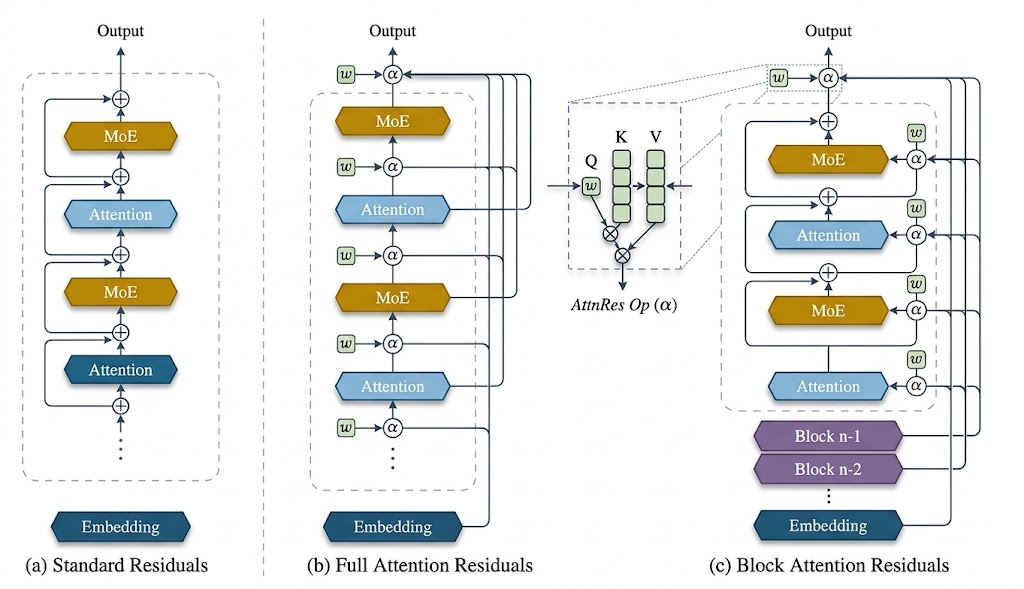
\includegraphics[width=0.8\textwidth]{VDT.jpg}
    \caption{Overview of Attention Residuals}
\end{figure}
\subsection{Three-sentence abstract-level story}


\subsection{Why this story is plausible}

The current repository already supports the exact ingredients needed for this thesis:

\begin{itemize}
  \item a preserved original baseline for historical reference,
  \item a same-stack \vanilla{} baseline for clean attribution,
  \item BAR and VCDR variants that differ only in actor-side depth routing,
  \item compute-aware depth infrastructure,
  \item offline-to-online tuning support aligned with the original \vdt{} narrative,
  \item RTG-grid reevaluation and routing-debug hooks for mechanism and alignment analysis.
\end{itemize}

\subsection{Why the story is not complete yet}

The story is promising but not yet paper-complete because the repository state alone is not the evidence. The paper still needs:

\begin{itemize}
  \item a convincing same-stack attribution result showing \texttt{BAR} beats \vanilla{} often enough to justify the architecture change,
  \item a convincing incremental result showing \texttt{state\_rtg\_value} improves on static BAR often enough to justify value-conditioned routing,
  \item a compute-aware depth story showing whether routing matters more when depth increases,
  \item and at least one stronger setting result, preferably online tuning, so the paper is not reduced to ``offline Gym architecture cosmetics''.
\end{itemize}

\begin{figure}[t]
\centering
\resizebox{0.97\textwidth}{!}{%
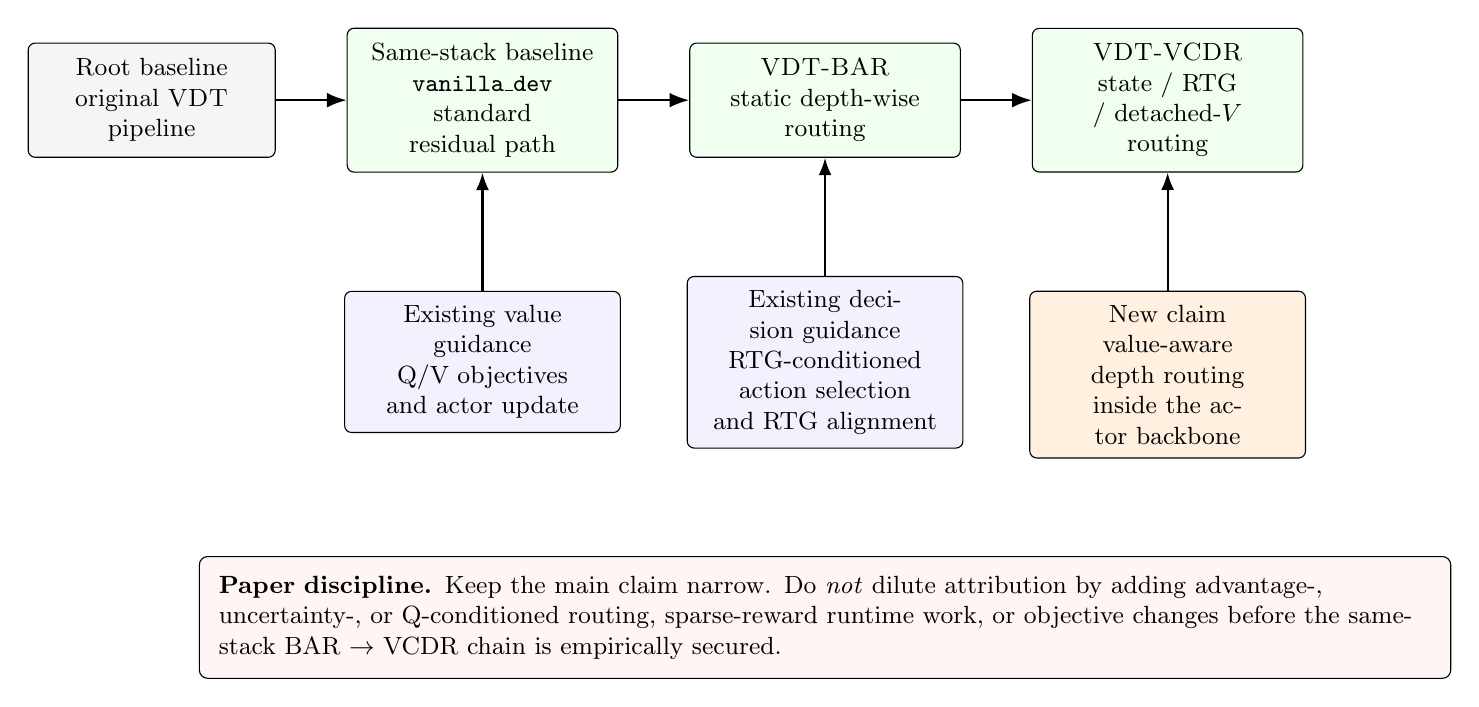
\begin{tikzpicture}[
  font=\small,
  node distance=10mm and 8mm,
  pipeline/.style={draw, rounded corners=2.5pt, align=center, text width=3.05cm, minimum height=1.45cm, inner sep=5.5pt, fill=green!6},
  baseline/.style={draw, rounded corners=2.5pt, align=center, text width=2.75cm, minimum height=1.45cm, inner sep=5.5pt, fill=gray!8},
  support/.style={draw, rounded corners=2.5pt, align=center, text width=3.15cm, minimum height=1.25cm, inner sep=5pt, fill=blue!5},
  claim/.style={draw, rounded corners=2.5pt, align=center, text width=3.15cm, minimum height=1.25cm, inner sep=5pt, fill=orange!12},
  note/.style={draw, rounded corners=3pt, align=left, text width=15.4cm, inner sep=7pt, fill=red!4},
  arrow/.style={-{Latex[length=2.5mm]}, thick},
  auxarrow/.style={-{Latex[length=2.2mm]}, thick}
]
  \node[baseline] (baseline) {Root baseline\\original \vdt{} pipeline};
  \node[pipeline, right=9mm of baseline] (van) {Same-stack baseline\\\vanilla{}\\standard residual path};
  \node[pipeline, right=9mm of van] (bar) {\barname{}\\static depth-wise\\routing};
  \node[pipeline, right=9mm of bar] (vcdr) {\vcdr{}\\state / RTG / detached-\(V\)\\routing};

  \draw[arrow] (baseline) -- (van);
  \draw[arrow] (van) -- (bar);
  \draw[arrow] (bar) -- (vcdr);

  \node[support, below=15mm of van] (obj) {Existing value guidance\\Q/V objectives\\and actor update};
  \node[support, below=15mm of bar] (rtg) {Existing decision guidance\\RTG-conditioned action selection\\and RTG alignment};
  \node[claim, below=15mm of vcdr] (route) {New claim\\value-aware depth routing\\inside the actor backbone};

  \draw[auxarrow] (obj.north) -- (van.south);
  \draw[auxarrow] (rtg.north) -- (bar.south);
  \draw[auxarrow] (route.north) -- (vcdr.south);

  \node[note, below=14mm of $(obj.south)!0.5!(route.south)$] (note) {
    \textbf{Paper discipline.} Keep the main claim narrow. Do \emph{not} dilute attribution by adding advantage-, uncertainty-, or Q-conditioned routing, sparse-reward runtime work, or objective changes before the same-stack BAR \(\rightarrow\) VCDR chain is empirically secured.
  };
\end{tikzpicture}
}
\caption{Repository-grounded paper framing. The proposal adds a third locus of value guidance---depth-wise routing---while preserving the original \vdt{} Q/V objectives and target-return semantics.}
\end{figure}

\section{What the Repository Already Secures for Publication}

\begin{tabularx}{\textwidth}{>{\raggedright\arraybackslash}p{0.21\textwidth}X}
\toprule
\textbf{Status} & \textbf{Assessment} \\
\midrule
\textbf{Strongest contribution} & Same-stack actor-side attribution: the repo now supports \vanilla{}, BAR, and VCDR under the same runner, checkpointing, manifest schema, aggregation, plotting, RTG-grid reevaluation, and online entrypoints. This is the clearest publishable asset because it isolates depth routing from unrelated engineering changes. \\
\textbf{Supporting contribution} & The project has become an experiment platform rather than a one-off model fork. Presets, manifests, compute reports, online/offline-aware aggregation, and routing-debug summaries make the work more reproducible and more reviewable. \\
\textbf{Still-weak contribution} & The structural depth claim is not yet strong until the matched-budget sweep is actually run and the compute overhead is reported next to returns. The infrastructure exists, but the paper value only materializes once the evidence is produced. \\
\textbf{Risky contribution} & Broad generality claims beyond Hopper medium are still weak. Sparse-reward claims are especially risky because Maze2D/AntMaze are only templates in the current runtime. Any main-text claim in that direction would currently overstate the repository. \\
\bottomrule
\end{tabularx}

\section{Reviewer-Style Direction Check}

\subsection{What the project is doing right}

\begin{itemize}
  \item The scope is disciplined: routing changes are isolated to the actor backbone.
  \item The same-stack baseline closes a major attribution gap that many architecture papers leave open.
  \item The online path makes the work more faithful to the original \vdt{} narrative than a pure offline-Gym-only paper.
  \item The analysis layer already supports RTG alignment, routing entropy, source usage, source distance, hidden norms, and query norms, which is unusually strong for mechanism follow-up.
\end{itemize}

\subsection{What could weaken the paper if not controlled}

\begin{itemize}
  \item If the paper tries to claim too many things at once---architecture, representation learning, sparse-reward stitching, online RL, and calibration---the core message will blur.
  \item If matched-budget evidence is missing, any strong ``deeper models benefit more'' claim will sound confounded by width and compute.
  \item If online results are weak, the paper should not force online as a headline contribution; it should become a supporting result or appendix line.
  \item If only Hopper is strong, the project must avoid pretending that the method is already a broad offline RL generalization story.
\end{itemize}

\subsection{What should \emph{not} expand right now}

\begin{itemize}
  \item Do not add advantage-conditioned routing yet.
  \item Do not add uncertainty-conditioned routing yet.
  \item Do not add Q-conditioned routing yet.
  \item Do not pivot the current paper around Maze2D or AntMaze until the runtime truly supports them.
  \item Do not let the paper become mostly about infrastructure; the infrastructure is a means to clean evidence, not the thesis.
\end{itemize}

\section{Critical Research Questions and Their Priority}

\begin{enumerate}
  \item \textbf{Same-stack attribution:} Does BAR beat \vanilla{} under the exact same dev stack? If not, the paper loses its first causal link.
  \item \textbf{Incremental routing value:} Does \texttt{state\_rtg\_value} beat static BAR reliably enough to justify conditioning routing on decision and value context?
  \item \textbf{Minimal useful dynamic context:} Is \texttt{state\_rtg\_value} actually better than \texttt{state} and \texttt{state\_rtg}, or is the detached value input unnecessary?
  \item \textbf{Depth story:} Does routing matter more as the actor gets deeper, especially when depth comparisons are compute-aware?
  \item \textbf{Online relevance:} Do BAR or VCDR improve offline-to-online tuning over the same-stack baseline, or are their gains confined to offline evaluation?
  \item \textbf{Alignment and mechanism:} Do RTG alignment curves and routing-mechanism summaries support the intended interpretation, rather than merely reporting return deltas?
\end{enumerate}

For the current repository, Questions 1 and 2 are \emph{mandatory}. Questions 3--5 are the main strengthening axes. Question 6 is critical for interpretation but should follow once the core behavioral signal exists.

\section{Staged Research Roadmap}

\subsection*{Stage A: Immediate (next 1--2 weeks)}

\textbf{Goal.} Establish whether the paper has a viable same-stack causal chain: \vanilla{} \(\rightarrow\) BAR \(\rightarrow\) VCDR.

\textbf{Must-run experiments.}
\begin{itemize}
  \item Hopper same-stack attribution: \vanilla{} vs.\ BAR static vs.\ VCDR \texttt{state\_rtg\_value}.
  \item Hopper query-mode sweep: \texttt{static}, \texttt{state}, \texttt{state\_rtg}, \texttt{state\_rtg\_value}.
  \item Hopper same-stack online compare: \vanilla{} vs.\ BAR vs.\ VCDR.
  \item One seed extension on the most promising same-stack and query-mode settings.
\end{itemize}

\textbf{Mechanism analysis.}
\begin{itemize}
  \item Routing entropy and source-distance summaries for BAR vs.\ VCDR.
  \item Query norm decomposition: static, delta, fused.
  \item RTG-grid reevaluation for at least BAR static vs.\ VCDR \texttt{state\_rtg\_value}.
\end{itemize}

\textbf{Deliverables.}
\begin{itemize}
  \item A first main-result table candidate for Hopper.
  \item A query-mode ablation figure.
  \item An initial online before/after bar figure.
  \item One alignment curve and one mechanism figure draft.
\end{itemize}

\textbf{Failure signals.}
\begin{itemize}
  \item BAR does not outperform \vanilla{} at all.
  \item VCDR fails to improve over BAR or only wins in noisy one-off seeds.
  \item Online results are flat or negative across all three variants.
\end{itemize}

\textbf{Go / no-go gate.}
\begin{itemize}
  \item \textbf{Go:} BAR \(>\) \vanilla{} on Hopper and VCDR \(>\) BAR on at least one meaningful axis (offline, online, or alignment).
  \item \textbf{No-go:} Neither causal step is supported. If that happens, narrow the paper immediately instead of expanding experiments.
\end{itemize}

\subsection*{Stage B: Decision and Expansion (2--6 weeks)}

\textbf{Goal.} Decide whether the paper can support a depth-routing story beyond a single-environment anecdote.

\textbf{Must-run experiments.}
\begin{itemize}
  \item Same-stack equal-width depth sweep: \vanilla{}, BAR, VCDR at 6/12/18 layers.
  \item Matched-budget depth sweep using the current preset generator.
  \item Gym same-stack environment sweep across Hopper, Walker2d, and HalfCheetah at 6 layers.
  \item Seed sweeps on the best one or two model families only.
\end{itemize}

\textbf{Mechanism analysis.}
\begin{itemize}
  \item Compare whether depth increases amplify routing selectivity or source-distance changes.
  \item Check whether VCDR's benefit tracks RTG alignment improvements.
  \item Build compute tables alongside return tables; never present deeper-is-better without compute context.
\end{itemize}

\textbf{Deliverables.}
\begin{itemize}
  \item A main-text table candidate across environments or across model families, depending on where the signal is strongest.
  \item A compute-aware depth figure and table.
  \item A refined mechanism panel for routing entropy, source usage, and query norms.
\end{itemize}

\textbf{Failure signals.}
\begin{itemize}
  \item Gains disappear outside Hopper.
  \item Depth claims vanish once budget matching is considered.
  \item The compute overhead is large enough that the return gains are not persuasive.
\end{itemize}

\textbf{Go / no-go gate.}
\begin{itemize}
  \item \textbf{Go:} at least one of the following becomes robust: cross-environment gains, compute-aware depth gains, or online gains.
  \item \textbf{No-go:} if the signal remains Hopper-only and shallow, reshape the paper around a narrower but cleaner claim.
\end{itemize}

\subsection*{Stage C: Manuscript Strengthening (paper convergence)}

\textbf{Goal.} Convert positive evidence into a compact, defensible conference paper.

\textbf{Main-text emphasis.}
\begin{itemize}
  \item Same-stack attribution must become the center of the narrative.
  \item One strengthening axis should accompany it in the main text: either online tuning, compute-aware depth, or RTG alignment/mechanism, depending on the strongest evidence.
\end{itemize}

\textbf{Appendix emphasis.}
\begin{itemize}
  \item Additional query-mode details.
  \item Full compute tables.
  \item Extra debug figures and per-layer visualizations.
  \item Extra seeds and supplementary environment breakdowns.
\end{itemize}

\textbf{Paper-writing gate.}
\begin{itemize}
  \item Lock the main table only after the same-stack and query-mode evidence are stable.
  \item Lock the main figure only after deciding which strengthening axis is strongest.
  \item Freeze algorithmic scope before drafting related work and final method sections.
\end{itemize}

\subsection*{Stage D: If the main conclusion is weak}

\textbf{Goal.} Preserve publishable value by narrowing the claim rather than over-claiming.

\textbf{Fallback pathways.}
\begin{itemize}
  \item If BAR beats \vanilla{} but VCDR is weak, write the paper as a depth-wise residual routing study with dynamic routing as an exploratory appendix result.
  \item If VCDR helps only online, position value-conditioned routing as a setting-sensitive extension rather than a universally better backbone.
  \item If the signal is narrow but interpretable, convert the paper into a mechanistic study of representation routing in value-guided decision models rather than a broad benchmark paper.
\end{itemize}

\section{Paper-Level Experiment Map}

\begin{longtable}{>{\raggedright\arraybackslash}p{0.18\textwidth} >{\raggedright\arraybackslash}p{0.20\textwidth} >{\raggedright\arraybackslash}p{0.17\textwidth} >{\raggedright\arraybackslash}p{0.13\textwidth} >{\raggedright\arraybackslash}p{0.22\textwidth}}
\toprule
\textbf{Experiment family} & \textbf{Repository support} & \textbf{Paper role} & \textbf{Priority} & \textbf{Placement} \\
\midrule
\endfirsthead
\toprule
\textbf{Experiment family} & \textbf{Repository support} & \textbf{Paper role} & \textbf{Priority} & \textbf{Placement} \\
\midrule
\endhead
Same-stack attribution & Dedicated launcher, manifests, checkpoints, aggregation & Establish BAR and VCDR as real improvements over the same-stack baseline & Mandatory now & Main text \\
Query-mode sweep & Dedicated 4-GPU launcher & Show whether detached value context matters beyond state and RTG & Mandatory now & Main text or main ablation \\
Online compare & Dedicated Hopper launcher plus online-aware aggregation/plotting & Show relevance to the original \vdt{} offline-to-online narrative & High priority & Main text if strong, appendix otherwise \\
Equal-width depth sweep & Existing preset/launcher support & Trend diagnostic for depth sensitivity & Important & Likely main text support or appendix, depending on signal \\
Matched-budget depth sweep & Preset generation plus compute tables & Structural rigor for the depth claim & High priority after Stage A & Main text if clean, appendix if mixed \\
RTG-grid reevaluation & Existing runner/eval path and plotting & Alignment/calibration evidence & Important but secondary & Main text support figure or appendix \\
Mechanism analysis & Debug hooks plus plotting scripts & Explain \emph{how} routing differs, not only \emph{whether} returns change & Important once returns move & Usually one main figure plus appendix extras \\
Sparse reward / trajectory stitching & Template only & Future extension or follow-up paper & Not current mainline & Not for current main text \\
\bottomrule
\end{longtable}

\section{Route from Now to Submission}

\begin{enumerate}
  \item \textbf{Run and aggregate the same-stack attribution line first.} This decides whether the paper can cleanly claim that actor-side depth routing helps at all.
  \item \textbf{Run query-mode sweep immediately after.} This decides whether the value-conditioned story is worth centering, or whether BAR alone is the real paper.
  \item \textbf{Inspect the first four artifacts before broad expansion:} the Hopper same-stack bar chart, the query-mode bar chart, the online before/after bar chart, and one RTG alignment curve.
  \item \textbf{Only then commit to the main strengthening axis.} If online looks strong, make online the paper's second pillar; if compute-aware depth looks stronger, make depth the second pillar instead.
  \item \textbf{Lock the main table once the same-stack and query-mode results are stable across seeds.}
  \item \textbf{Add mechanism figures only after the behavioral result is fixed.} Mechanism plots are supporting evidence; they should not be used to rescue a weak main result.
  \item \textbf{Decide by manuscript time whether harder extensions are worth it.} Sparse reward, extra routing channels, or broader online work should only continue if the core paper is already secure.
\end{enumerate}

\section{Risks and Backup Plans}

\begin{tabularx}{\textwidth}{>{\raggedright\arraybackslash}p{0.27\textwidth}X}
\toprule
\textbf{Risk} & \textbf{Response} \\
\midrule
BAR does not beat \vanilla{} & Do not keep a broad routing paper. Either narrow to an exploratory negative result plus mechanism observations, or terminate the BAR/VCDR mainline and avoid building on a broken first link. \\
VCDR does not beat BAR & Reframe VCDR as an exploratory extension. The current paper can still be a clean BAR paper if same-stack BAR is robust. \\
Online tuning shows no gain & Keep online as a secondary evaluation line rather than a central claim. Use it to show compatibility, not superiority. \\
Only some environments improve & State the scope honestly. A strong Hopper story with clear attribution can still be publishable if the mechanism is convincing and the claims are appropriately narrow. \\
Compute overhead is too high & Pair every depth claim with compute tables. If compute-normalized value is weak, downgrade the depth claim and foreground same-stack attribution instead. \\
Mechanism plots are noisy or non-diagnostic & Keep only one or two clean mechanism figures in the paper; move the rest to appendix rather than overfitting interpretation. \\
\bottomrule
\end{tabularx}

\section{Most Recommended Next Actions}

\begin{enumerate}
  \item \textbf{Complete Hopper same-stack attribution.} Purpose: verify the first causal link. Success criterion: BAR meaningfully exceeds \vanilla{} and VCDR is at least competitive with or better than BAR.
  \item \textbf{Complete Hopper query-mode sweep and one seed extension.} Purpose: verify whether the detached value channel is a real contributor. Success criterion: \texttt{state\_rtg\_value} is best or tied-best with cleaner RTG/mechanism behavior than simpler modes.
  \item \textbf{Complete Hopper online compare and at least one RTG-grid alignment pass.} Purpose: determine whether the paper's second pillar should be online relevance or something else. Success criterion: one of online gains, alignment gains, or compute-aware depth gains becomes clearly worth main-text emphasis.
\end{enumerate}

\paragraph{Bottom line.}
This repository is already beyond the stage of asking ``what could we try?'' The right question now is ``what is the narrowest, strongest conference paper that the current stack can support?'' The answer is not a sprawling new-method paper. It is a disciplined same-stack depth-routing paper in which BAR establishes the architectural effect, VCDR tests whether decision/value context improves routing further, and one carefully chosen strengthening axis---online tuning, compute-aware depth, or alignment/mechanism---turns a neat idea into a credible submission.

\end{document}
